% TextEditor+ User Manual
%
% Build with XeLaTeX or LuaLaTeX (the key symbols need a Unicode engine):
%   tectonic TextEditor+-User-Manual.tex
%   or: xelatex TextEditor+-User-Manual.tex  (run twice for the contents)

\documentclass[11pt,a4paper]{article}

\usepackage{fontspec}
\usepackage[margin=2.5cm]{geometry}
\usepackage{graphicx}
\usepackage{xcolor}
\usepackage{booktabs}
\usepackage{tabularx}
\usepackage{array}
\usepackage{enumitem}
\usepackage{titlesec}
\usepackage{fancyhdr}
\usepackage[skins,breakable]{tcolorbox}
\usepackage[hidelinks]{hyperref}

% Fonts are loaded by file name so the file builds with Tectonic, which
% can't look fonts up by family name.
\setmainfont{texgyrepagella}[Extension=.otf, UprightFont=*-regular,
  BoldFont=*-bold, ItalicFont=*-italic, BoldItalicFont=*-bolditalic]
\setsansfont{texgyreheros}[Extension=.otf, UprightFont=*-regular,
  BoldFont=*-bold, ItalicFont=*-italic, BoldItalicFont=*-bolditalic]
\setmonofont{DejaVuSansMono}[Extension=.ttf, UprightFont=*, BoldFont=*-Bold,
  ItalicFont=*-Oblique, BoldItalicFont=*-BoldOblique, Scale=MatchLowercase]
% DejaVu Sans has the Mac key symbols (⌘ ⌥ ⇧ ⌃) that the text fonts lack.
\newfontfamily\keyfont{DejaVuSans.ttf}[Scale=0.85]

\definecolor{accent}{HTML}{6C4AB6}
\definecolor{keybg}{HTML}{F1F1F4}
\definecolor{keyframe}{HTML}{B9B9C3}
\definecolor{notebg}{HTML}{F4F0FB}
\definecolor{warnbg}{HTML}{FFF4E5}
\definecolor{warnframe}{HTML}{E0A040}

\hypersetup{
  pdftitle={TextEditor+ User Manual},
  pdfauthor={Sanjeeva Wijeyesakere},
  pdfsubject={User manual for TextEditor+ 3.0.0},
}

\newcommand{\appname}{TextEditor+}
\newcommand{\version}{3.0.0}

% A key or key combination, drawn as a keycap: \key{⌘S}, \key{Ctrl+S}.
\newtcbox{\key}{on line, nobeforeafter, boxrule=0.4pt, arc=2pt,
  colback=keybg, colframe=keyframe,
  left=2.5pt, right=2.5pt, top=0.5pt, bottom=0.5pt,
  fontupper=\keyfont}
% A menu path: \menu{File > Save As…}
\newcommand{\menu}[1]{\textsf{\textbf{#1}}}
\newcommand{\ui}[1]{\textsf{#1}}

\newtcolorbox{note}[1][Note]{enhanced, breakable, colback=notebg, colframe=accent,
  boxrule=0pt, leftrule=3pt, arc=0pt, left=8pt, right=8pt, top=4pt, bottom=4pt,
  fonttitle=\sffamily\bfseries\color{accent}, coltitle=accent, colbacktitle=notebg,
  title=#1, attach title to upper={\ \ }}
\newtcolorbox{caution}[1][Caution]{enhanced, breakable, colback=warnbg, colframe=warnframe,
  boxrule=0pt, leftrule=3pt, arc=0pt, left=8pt, right=8pt, top=4pt, bottom=4pt,
  fonttitle=\sffamily\bfseries, coltitle=warnframe!70!black, colbacktitle=warnbg,
  title=#1, attach title to upper={\ \ }}

\titleformat{\section}{\sffamily\Large\bfseries\color{accent}}{\thesection}{0.8em}{}
\titleformat{\subsection}{\sffamily\large\bfseries}{\thesubsection}{0.8em}{}
\titleformat{\subsubsection}{\sffamily\normalsize\bfseries}{}{0em}{}

\pagestyle{fancy}
\fancyhf{}
\fancyhead[L]{\sffamily\small\appname\ User Manual}
\fancyhead[R]{\sffamily\small Version \version}
\fancyfoot[C]{\sffamily\small\thepage}
\renewcommand{\headrulewidth}{0.4pt}

\setlist{itemsep=2pt, topsep=4pt}
\setlength{\parskip}{4pt}
\renewcommand{\arraystretch}{1.25}

\begin{document}

% ---------------------------------------------------------------- Title page
\hypersetup{pageanchor=false}
\begin{titlepage}
  \centering
  \vspace*{3cm}
  
\includegraphics[width=3cm]{figures/icon.png}\par
  \vspace{1cm}
  {\sffamily\fontsize{36}{40}\selectfont\bfseries \appname\par}
  \vspace{0.4cm}
  {\sffamily\LARGE User Manual\par}
  \vspace{0.6cm}
  {\sffamily\large Version \version\par}
  \vfill
  {\large A lightweight code and text editor for macOS, Windows and Linux\par}
  \vspace{1.5cm}
  {\sffamily Sanjeeva Wijeyesakere\par}
  {\sffamily\small \href{https://sjwrc.com}{sjwrc.com} \quad·\quad
   \href{https://github.com/swijeyes}{github.com/swijeyes}\par}
  \vspace{0.5cm}
  {\sffamily\small October 2026\par}
\end{titlepage}
\hypersetup{pageanchor=true}

{\setlength{\parskip}{0pt}\tableofcontents}
\clearpage

% ---------------------------------------------------------------- Introduction
\section{Introduction}

\appname\ is a fast, lightweight editor for code and plain text. It is the
native desktop version of
\href{https://sjwrc.com/tools/editor/}{Web TextEditor}, the browser-based editor
on sjwrc.com, and keeps its look and features while adding your operating
system's own file dialogs, printing, find and replace, and more.

\appname\ is built for quick edits: it opens instantly and stays out of your
way. Its main features are:

\begin{itemize}
  \item \textbf{Tabs and folders} (new in 2.0): open several files at once,
        each in its own tab, and browse a folder in the sidebar.
  \item \textbf{Files on servers} (new in 2.0): open, edit and save files
        and folders on any SFTP server, using your existing SSH keys.
  \item \textbf{Syntax highlighting} for HTML (including embedded
        \texttt{<script>} and \texttt{<style>} sections), CSS, JavaScript, C,
        C++, and (new in 2.5) Markdown, Python, Rust and \LaTeX, chosen
        automatically from the file name.
  \item \textbf{Live preview} (new in 2.5): \LaTeX, Markdown and HTML
        documents are shown formatted beside the text as you type
        (section~\ref{sec:texpreview}).
  \item \textbf{Grid view for CSV and TSV} (new in 3.0): switch a
        comma- or tab-separated file to a spreadsheet-style grid with
        sorting, filtering, search and formulas --- arithmetic, statistical,
        financial, logical and text functions (section~\ref{sec:grid}).
  \item \textbf{Classic scroll bars} (new in 2.5): a glossy blue thumb,
        with both arrow buttons together at the end.
  \item \textbf{Two colour themes}: Dark and Light.
  \item \textbf{Colourful toolbar icons and Settings} (new in 2.5): choose
        how the toolbar looks and which buttons it shows, the theme, line
        numbers and spell checking (section~\ref{sec:settings}).
  \item \textbf{Spell checking} (new in 2.5) with your system's dictionary,
        in text, comments and strings (section~\ref{sec:spelling}).
  \item \textbf{Comfortable editing}: line numbers, current-line highlight,
        automatic indentation, word wrap and Go to Line.
  \item \textbf{Find and replace} with case matching, whole-word search,
        regular expressions and back-references.
  \item \textbf{Faithful saving}: every file keeps its line endings and
        encoding, and saves are atomic, so a failed save never leaves a
        half-written file.
  \item \textbf{Printing} of a whole file or a selection, in colours suited
        to paper.
  \item \textbf{Safeguards} against opening devices, binary files and very
        large files by accident, and a warning before saving over changes
        someone else made.
\end{itemize}

\subsection{About this manual}

This manual covers \appname\ \version. Keyboard shortcuts are given for macOS
first and for Windows and Linux second, for example \key{⌘S} / \key{Ctrl+S}.
On a Mac, \key{⌘} is the Command key, \key{⌥} is Option, \key{⇧} is Shift and
\key{⌃} is Control. Menu commands are written as \menu{File > Save As…}.

% ---------------------------------------------------------------- Installing
\section{Installing \appname}

\subsection{macOS}\label{sec:install-mac}

\appname\ for macOS is distributed as a disk image,
\texttt{TextEditor+-\version.dmg}, for Apple Silicon (M-series) Macs.

\begin{enumerate}
  \item Double-click \texttt{TextEditor+-\version.dmg} to open it.
  \item Drag \textbf{\appname} onto the \textbf{Applications} folder shown in
        the same window.
  \item Eject the disk image.
\end{enumerate}

The current build is not notarised by Apple, so macOS blocks the first launch
with a message that it cannot verify the app. To open it the first time,
either:

\begin{itemize}
  \item \textbf{Control-click} (or right-click) \appname\ in the Applications
        folder, choose \menu{Open}, and confirm with \ui{Open}; or
  \item try to open it normally, then go to \menu{System Settings > Privacy \&
        Security} and click \ui{Open Anyway}.
\end{itemize}

You only need to do this once. After that, \appname\ opens like any other app.

\subsection{Windows}\label{sec:install-windows}

\appname\ for Windows is a portable app for 64-bit Windows 10 and 11,
distributed as a zip file,
\texttt{TextEditor+-\version-windows-x64.zip}. It needs no installation.

\begin{enumerate}
  \item Extract the whole folder from the zip file to wherever you like: your
        Documents folder, the desktop or a USB stick. Don't run \appname\ from
        inside the zip file.
  \item Double-click \texttt{TextEditor+.exe} in the extracted folder.
\end{enumerate}

The program isn't signed, so the first time you run it Windows SmartScreen may
say ``Windows protected your PC''. Click \ui{More info}, then \ui{Run anyway}.

The portable version keeps its settings in the \texttt{settings} folder next to
\texttt{TextEditor+.exe} rather than in the Windows registry, so they travel
with the folder. Besides the window and editor settings, this includes your
open tabs and sidebar folder, the Open Recent list and your saved servers, but
never a password. That folder must be writable for settings to be saved. If you
delete the \texttt{settings} folder, \appname\ stores its settings in the
registry like an installed program.

To remove \appname, delete its folder. Nothing else was installed; a server key
you chose to trust stays in your \texttt{.ssh\textbackslash known\_hosts} file, as
it would for the \texttt{ssh} command.

The folder also contains \texttt{README.txt}, this manual, and a
\texttt{licenses} folder with the licences of \appname\ and the libraries it
includes (Qt, libssh, OpenSSL and the LLVM and MinGW runtime libraries).

\subsection{Linux}

There are no prebuilt packages for Linux yet. \appname\ can be built from
source with Qt~6.4 or later, CMake~3.21 or later, a C++17 compiler and, for
SFTP, libssh~0.11.5 or later; the
\texttt{README.md} file in the source code has step-by-step instructions.

\begin{note}
Everything in this manual applies to all three platforms unless a section says
otherwise. A few behaviours, such as dropping files on the Dock icon, exist only
on macOS.
\end{note}

% ---------------------------------------------------------------- Tour
\section{A tour of the window}

\begin{figure}[h]
  \centering
  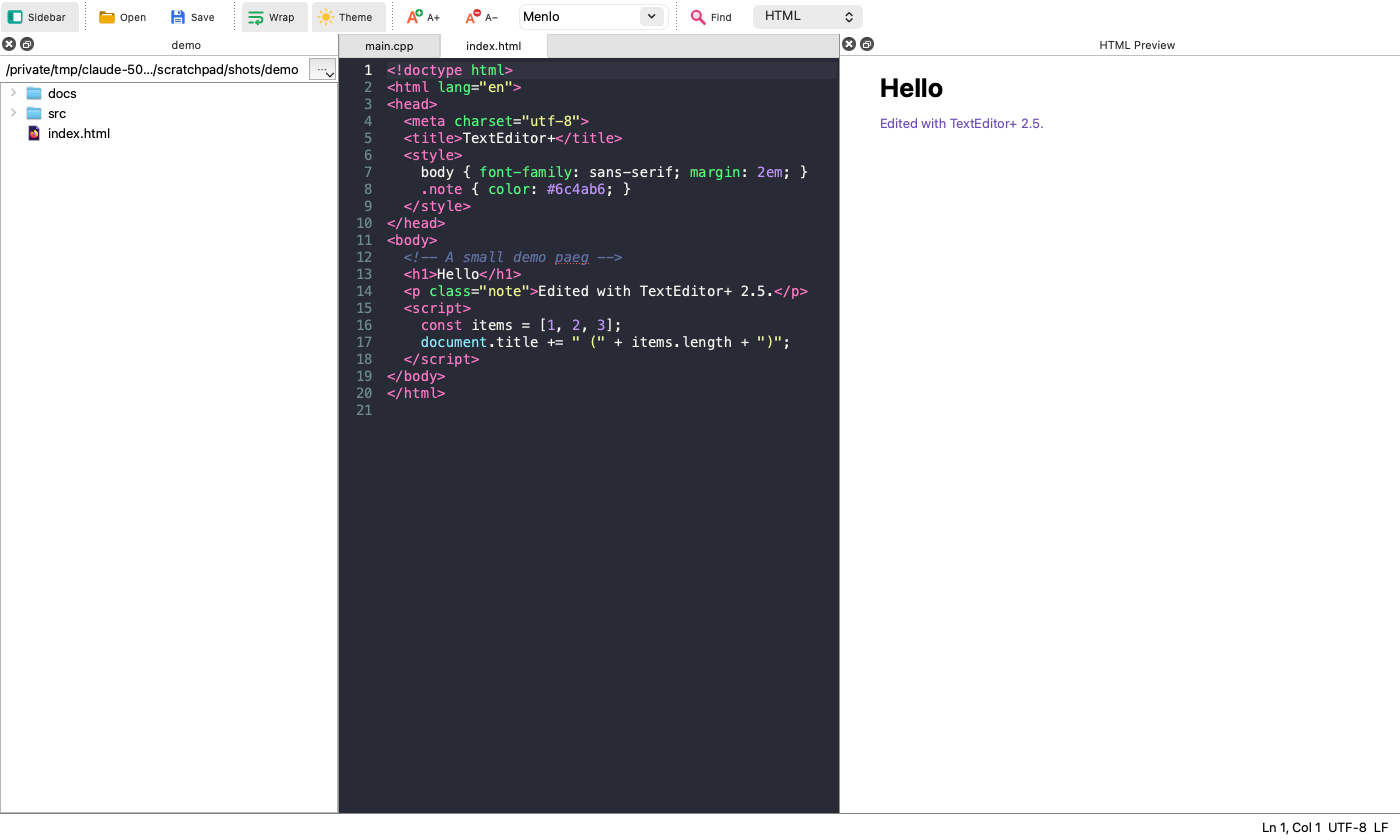
\includegraphics[width=\linewidth]{figures/screenshot.png}
  \caption{\appname\ with a folder open in the sidebar and two files in tabs.}
  \label{fig:window}
\end{figure}

The \appname\ window (Figure~\ref{fig:window}) has a toolbar, a row of
tabs, one for each open file, the editing area, a status bar and, when you open
a folder, a sidebar listing its files (section~\ref{sec:folders}).

\subsection{The toolbar}

Each toolbar button has a coloured icon with its name beside it. From left to
right, the toolbar holds:

\begin{center}
\begin{tabularx}{\linewidth}{>{\sffamily}l X}
  \toprule
  \textbf{Control} & \textbf{What it does} \\
  \midrule
  Sidebar     & Shows or hides the folder sidebar (section~\ref{sec:folders}). \\
  Open        & Opens a file (section~\ref{sec:opening}). \\
  Save        & Saves the current file (section~\ref{sec:saving}). \\
  Wrap        & Turns word wrap on or off. Highlighted when on. \\
  Theme       & Switches between the dark and light themes. Highlighted when the
                dark theme is on. \\
  A+ \quad A− & Makes the text larger or smaller. \\
  Font box    & Chooses the editor font. Only monospaced (fixed-width) fonts
                are listed. \\
  Find        & Opens the find bar (section~\ref{sec:find}). \\
  Language box & Chooses the syntax highlighting (section~\ref{sec:languages}). \\
  \bottomrule
\end{tabularx}
\end{center}

The Theme button shows a sun in the dark theme and a moon in the light one:
the theme it switches to. In Settings (section~\ref{sec:settings}) you can put
the names under the icons or show the icons alone, and hide buttons you don't
use. Point at a button to see its name and keyboard shortcut. Hidden buttons'
commands stay in the menus.

\subsection{Tabs}\label{sec:tabs}

Each open file has its own tab above the editing area, showing the file's
name. A dot (•) after the name means the file has unsaved changes. Point at a
tab to see the file's full path, or its \texttt{sftp://} address for a file on
a server.

\begin{itemize}
  \item Click a tab to switch to it, or press \key{⌃Tab} / \key{Ctrl+Tab}
        for the next tab and \key{⌃⇧Tab} / \key{Ctrl+⇧Tab} for the previous
        one.
  \item Drag a tab to move it.
  \item Close a tab with its close button, \menu{File > Close Tab} or
        \key{⌘W} / \key{Ctrl+W}. Closing the last tab leaves an empty,
        untitled one.
  \item \menu{File > New Tab} (\key{⌘N} / \key{Ctrl+N}, or \key{⌘T} /
        \key{Ctrl+T}) opens a tab for a new file.
\end{itemize}

Menu commands, the find bar, the status bar and the language box always apply
to the tab you are looking at. The theme, font, text size and word wrap apply
to all tabs.

\subsection{The editing area}

The editing area shows your text with line numbers on the left (you can turn
them off in Settings). The line containing the cursor is highlighted, and its
line number is drawn in a brighter colour. Misspelled words are underlined with
a red dotted line (section~\ref{sec:spelling}).

The scroll bars are drawn in the \appname\ ``Classic'' style, on every
platform: a glossy blue thumb that turns grey while the window is in the
background, and both arrow buttons together at the bottom (or right-hand) end.
Click an arrow to scroll a line, click the track to scroll a page, or drag the
thumb. In the dark theme the track and buttons are dark too.

\subsection{The status bar}

The status bar along the bottom shows, from left to right:

\begin{itemize}
  \item the cursor position, as \ui{Ln} (line) and \ui{Col} (column);
  \item the file's text encoding, \ui{UTF-8} or \ui{Latin-1};
  \item the file's line endings, \ui{LF} (macOS and Linux style) or \ui{CRLF}
        (Windows style).
\end{itemize}

Short messages, such as ``Saved notes.txt'', also appear briefly on the left of
the status bar.

\subsection{The title bar}

The title bar shows the name of the current tab's file, or \ui{Untitled} for a
new one. For a file on a server, it also shows the server's name.
When the file has unsaved changes, macOS shows a dot in the window's close
button, and Windows and Linux add an asterisk (*) after the name.

% ---------------------------------------------------------------- Opening
\section{Opening files}\label{sec:opening}

Each file you open gets its own tab (section~\ref{sec:tabs}). If the file is
already open, \appname\ switches to its tab instead of opening it twice. If the
current tab is an empty, untitled one, the file opens in it.

\subsection{Ways to open a file}

\begin{description}[style=nextline, leftmargin=1.5em]
  \item[Open dialog]
    Choose \menu{File > Open…}, press \key{⌘O} / \key{Ctrl+O}, or click
    \ui{Open} in the toolbar. The dialog starts in the folder of the file you
    have open. You can choose several files at once; each opens in its own
    tab. Use the file-type menu in the dialog to show only text, web or C/C++
    files.
  \item[The sidebar]
    Click a file in the folder sidebar (section~\ref{sec:folders}).
  \item[Open Recent]
    \menu{File > Open Recent} lists the files and folders you opened lately,
    on this computer and on servers. \menu{Clear Menu} empties the list.
  \item[Drag onto the window]
    Drag a file from Finder, File Explorer or your file manager and drop it
    anywhere on the editing area. Dropping a folder opens it in the sidebar.
  \item[Drag onto the Dock icon (macOS)]
    Drop a file on the \appname\ icon in the Dock. This works whether or not
    \appname\ is already running. Dropping a folder opens it in the sidebar.
  \item[Open With (macOS)]
    In Finder, Control-click a file and choose
    \menu{Open With > \appname}. \appname\ is listed for every file but never
    makes itself the default app for any file type, so double-clicking files
    keeps opening them in your usual apps.
  \item[Command line]
    Pass file or folder names when starting the program, for example
    \texttt{TextEditor+ notes.txt todo.md}, or \texttt{sftp://} addresses such
    as \path{TextEditor+ sftp://alice@example.com/var/www/index.html}. Run \texttt{TextEditor+ -{}-help} for the
    options, or \texttt{-{}-version} to print the version.
\end{description}

When you open a file, \appname\ picks the syntax highlighting from its file
extension (section~\ref{sec:languages}).

\subsection{Safeguards when opening}

To protect you from mistakes, \appname\ checks each file before opening it:

\begin{itemize}
  \item \textbf{Only regular files are opened.} Folders, devices and pipes are
        refused with a message, because reading them could never finish.
  \item \textbf{Binary files need confirmation.} If a file contains NUL bytes,
        which text files do not, \appname\ warns that it appears to be binary
        and asks whether to open it anyway.
  \item \textbf{Large files need confirmation.} Files over 50~MB can make the
        editor slow, so you are asked before they open.
  \item \textbf{Very large files are refused.} Files over 512~MB are not
        opened at all, because the whole file is held in memory.
  \item \textbf{Symbolic links are reported.} If the file is a symbolic link
        (alias), a message in the status bar names the file it points to;
        saving writes to that file and leaves the link in place.
\end{itemize}

The same checks apply to files on a server.

\begin{caution}
Saving a binary file from a text editor usually damages it. Open binary files
only to look at them, and close them without saving.
\end{caution}

\subsection{Encodings}

\appname\ reads files as UTF-8, the standard encoding for modern text. If a file
is not valid UTF-8, it is opened as Latin-1 (ISO 8859-1) instead, the status bar
shows \ui{Latin-1}, and a message ``Not valid UTF-8: opened as Latin-1'' appears
for a few seconds. Section~\ref{sec:saving} explains how the encoding is kept
when you save.

% ---------------------------------------------------------------- Editing
\section{Editing text}

\appname\ supports the standard editing commands of your platform: typing,
selecting with the mouse or with \key{⇧} and the arrow keys, and the usual
clipboard commands.

\subsection{The Edit menu}

\begin{center}
\begin{tabularx}{\linewidth}{>{\sffamily}l l l X}
  \toprule
  \textbf{Command} & \textbf{macOS} & \textbf{Windows / Linux} & \textbf{Notes} \\
  \midrule
  Undo       & \key{⌘Z}  & \key{Ctrl+Z} & Unavailable when there is nothing to undo. \\
  Redo       & \key{⇧⌘Z} & \key{Ctrl+Y} or \key{Ctrl+⇧Z} & \\
  Cut        & \key{⌘X}  & \key{Ctrl+X} & \\
  Copy       & \key{⌘C}  & \key{Ctrl+C} & \\
  Paste      & \key{⌘V}  & \key{Ctrl+V} & Always pastes plain text. \\
  Select All & \key{⌘A}  & \key{Ctrl+A} & \\
  \bottomrule
\end{tabularx}
\end{center}

\subsection{Automatic indentation}

When you press \key{Return} / \key{Enter}, the new line starts with the same
indentation (spaces and tabs) as the line above, so code stays lined up.
Tab stops are four characters wide.

\subsection{Go to Line}

Choose \menu{Edit > Go to Line…} or press \key{⌘L} / \key{Ctrl+L}, type a line
number, and press \key{Return}. The dialog shows the range of valid line numbers,
and the line you choose is scrolled to the middle of the window.

\subsection{Spelling}\label{sec:spelling}

\appname\ underlines misspelled words with a red dotted line as you type. It
checks the words people read, not code:

\begin{itemize}
  \item all of a plain-text file;
  \item the text of Markdown, HTML and \LaTeX\ files (not code spans, tags,
        commands or maths);
  \item comments and strings in program code.
\end{itemize}

Words that look like code are skipped: \texttt{camelCase} and
\texttt{snake\_case} names, words joined to digits, words in capitals such as
\texttt{HTML}, single letters, and anything in a web address, e-mail address or
file path.

Right-click an underlined word for suggestions; choose one to replace the
word. \ui{Ignore Spelling} accepts the word until you quit \appname.
\ui{Add to Dictionary} adds it to your own dictionary for good.

The dictionary is your system's own, so it follows your language settings, and
words you add are shared with other apps:

\begin{itemize}
  \item \textbf{macOS}: the languages in \menu{System Settings > Keyboard >
        Text Input > Edit > Spelling} (\ui{Automatic by Language} by default).
  \item \textbf{Windows}: your Windows display language, or US English if
        Windows has no dictionary for it. Add a language's spelling under
        \menu{Settings > Time \& language > Language \& region}.
  \item \textbf{Linux}: spell checking isn't available yet.
\end{itemize}

Turn spell checking off in Settings (section~\ref{sec:settings}).

% ---------------------------------------------------------------- Find
\section{Find and replace}\label{sec:find}

\subsection{Finding text}

Choose \menu{Edit > Find…}, press \key{⌘F} / \key{Ctrl+F}, or click \ui{Find}
in the toolbar. The find bar opens above the text. If you had selected some text
on a single line, it is filled in for you.

As you type, \appname\ jumps to the first match from the cursor. Then:

\begin{itemize}
  \item press \key{Return} or click \ui{Next} to go to the next match;
  \item press \key{⇧Return} or click \ui{Previous} to go to the previous match;
  \item press \key{Esc} or click \ui{{\keyfont ✕}} to close the find bar.
\end{itemize}

You can also use \menu{Edit > Find Next} (\key{⌘G} / \key{F3}) and
\menu{Edit > Find Previous} (\key{⇧⌘G} / \key{⇧F3}) with the find bar closed.
Searching wraps around: after the last match it continues from the top of the
file. If nothing matches, the find bar shows \ui{No matches} in red.

\subsection{Search options}

\begin{description}[leftmargin=1.5em]
  \item[\ui{Match case}] Only finds text with the same capitalisation;
    ``Hello'' no longer matches ``hello''.
  \item[\ui{Whole word}] Only finds complete words; ``cat'' no longer matches
    inside ``concatenate''.
  \item[\ui{Regex}] Treats the search text as a regular expression
    (section~\ref{sec:regex}).
\end{description}

\subsection{Replacing text}

Choose \menu{Edit > Replace…} or press \key{⌥⌘F} on macOS, \key{Ctrl+H} on
Windows and most Linux desktops, or \key{Ctrl+R} on KDE. The find bar opens with
the cursor in the \ui{Replace with} box. Then:

\begin{itemize}
  \item \ui{Replace} (or \key{Return} in the \ui{Replace with} box) replaces the
        selected match and moves on to the next one;
  \item \ui{Replace All} replaces every match in the file and reports how many
        it replaced.
\end{itemize}

A \ui{Replace All} can be undone in one step with \menu{Edit > Undo}.

\subsection{Regular expressions}\label{sec:regex}

With \ui{Regex} ticked, the search text is a Perl-compatible regular
expression. For example:

\begin{center}
\begin{tabularx}{\linewidth}{>{\ttfamily}l X}
  \toprule
  \textbf{\textsf{Pattern}} & \textbf{Finds} \\
  \midrule
  \textbackslash d+           & one or more digits, such as \texttt{42} \\
  colou?r                     & ``color'' or ``colour'' \\
  \textasciicircum\textbackslash s+\$ & lines that contain only spaces or tabs \\
  (\textbackslash w+)@(\textbackslash w+) & a word, an @ sign and another word \\
  \bottomrule
\end{tabularx}
\end{center}

In the \ui{Replace with} box, \texttt{\textbackslash 1}, \texttt{\textbackslash 2}
and so on insert the text matched by the first, second, \ldots\ group in
parentheses. For example, searching for
\texttt{(\textbackslash w+)@(\textbackslash w+)} and replacing with
\texttt{\textbackslash 2 at \textbackslash 1} turns \texttt{alice@example} into
\texttt{example at alice}.

If the pattern is not a valid regular expression, the find bar shows
\ui{Invalid pattern} and nothing is searched or replaced.

\begin{note}
Matches cannot span more than one line.
\end{note}

% ---------------------------------------------------------------- Languages
\section{Syntax highlighting}\label{sec:languages}

\appname\ colours keywords, strings, numbers, comments and other parts of the
text to make code easier to read. The highlighting language is chosen from the
file extension when you open or save a file:

\begin{center}
\begin{tabularx}{\linewidth}{>{\sffamily}l X}
  \toprule
  \textbf{Language} & \textbf{File extensions} \\
  \midrule
  HTML       & \texttt{.html .htm .xhtml .xml .svg .vue} \\
  CSS        & \texttt{.css .scss .less} \\
  JavaScript & \texttt{.js .mjs .cjs .jsx .ts .tsx .json} \\
  C          & \texttt{.c .h} \\
  C++        & \texttt{.cpp .cc .cxx .hpp .hh .hxx .ino} \\
  Markdown   & \texttt{.md .markdown .mdown .mkd .mdx} \\
  Python     & \texttt{.py .pyw .pyi} \\
  Rust       & \texttt{.rs} \\
  LaTeX      & \texttt{.tex .latex .ltx .sty .cls} \\
  Plain Text & anything else \\
  \bottomrule
\end{tabularx}
\end{center}

In HTML files, the contents of \texttt{<script>} and \texttt{<style>} sections
are highlighted as JavaScript and CSS.

To choose a language yourself, use the \menu{Language} menu or the language box
in the toolbar. Your choice applies until you open another file. Saving under a
new name with a recognised extension switches to that extension's language;
saving under a name the table doesn't list, such as \texttt{notes.txt}, keeps
your choice.

% ---------------------------------------------------------------- Preview
\section{The live preview}\label{sec:texpreview}

When the current tab holds a \LaTeX, Markdown or HTML document, a preview
appears in a sidebar on the right. It follows your typing, including changes
you haven't saved, and hides again when you switch to a file it can't show.
Drag its edge to make it wider or narrower. The preview's title says what it
is showing: \ui{TeX Preview}, \ui{Markdown Preview} or \ui{HTML Preview}.

\subsection{Markdown}

Markdown files (\texttt{.md}, \texttt{.markdown} and similar, or any tab whose
language you set to Markdown) are shown formatted, in the colours of the
current theme: headings, emphasis, lists and task lists, quotes, code (shaded),
tables, links and images. GitHub-flavoured Markdown is understood.

\subsection{HTML}

HTML files (\texttt{.html}, \texttt{.htm} and \texttt{.xhtml}, or any tab whose
language you set to HTML) are shown as a web page, black on white as a
browser shows it unless the page sets its own colours. Style sheets in
\texttt{<style>} sections, \texttt{style} attributes and \texttt{.css} files
linked from the file's folder are applied, and images in the file's folder
(or embedded as \texttt{data:} addresses) are shown. XML, SVG and Vue files,
which are highlighted as HTML, have no preview.

The page is drawn by \appname\ itself rather than a web browser, so it is a
preview of the page's content and styling, not an exact rendering: scripts
don't run, CSS layout (such as flexbox, grid and positioning) is simplified,
and nothing is ever fetched from the internet, so web fonts, remote images
and remote style sheets are left out. Clicking a web link opens it in your
browser.

\subsection{\LaTeX}

When the current tab holds a \LaTeX\ document (a \texttt{.tex}, \texttt{.latex}
or \texttt{.ltx} file, or any tab whose language you set to \LaTeX), the menu
at the top of the preview chooses how it is made:

\begin{description}
  \item[Quick Preview] needs nothing else installed and updates as you type.
    It shows the title, sections and table of contents, lists, tables,
    figures and images, footnotes, cross-references and citations, theorems
    and proofs, verbatim text and your own \verb|\newcommand| macros. Maths is
    drawn with proper symbols, superscripts and subscripts, and equations are
    numbered. It is an approximation: complicated maths, page layout and
    pictures drawn with TikZ appear only when typeset.
  \item[Typeset with \ldots] appears for each \TeX\ engine found on your
    computer: pdf\LaTeX, Xe\LaTeX, Lua\LaTeX\ (from MacTeX, \TeX~Live or MiK\TeX)
    or Tectonic. A moment after you stop typing, the document is typeset and
    its pages are shown exactly as they will print (the first 40 pages). If
    the document has an error, the first one is shown above the pages, with
    its line number. \ui{Open PDF} opens the typeset PDF in your PDF viewer.
    The pages are drawn with Poppler's \texttt{pdftoppm} or MuPDF's
    \texttt{mutool}; without either, use \ui{Open PDF}.
\end{description}

When both a \TeX\ engine and a PDF renderer are installed, the preview starts
in Typeset mode; otherwise it starts in Quick Preview. Your choice is
remembered.

\begin{note}
Typesetting starts as soon as you open a file, so it is kept safe even for
documents you didn't write. It uses a private temporary folder, so nothing is
written next to your file, and \TeX's shell escape is always off. On macOS and
Linux, \TeX\ also runs in a sandbox that stops it writing anywhere else or
using the network (Tectonic may still download packages). Tectonic and
Lua\LaTeX\ are offered only where there is such a sandbox. Files that the
document loads from its own folder, such as images and \verb|\input| files,
are still found. Tectonic downloads the packages a document needs the first
time it uses them, so the first preview can take a little while.
\end{note}

\subsection{Closing the preview}

To close the preview, click its close button; it then stays closed for all
files until you choose \menu{View > Show Preview}
(\key{⇧⌘P} / \key{Ctrl+⇧P}).

% ---------------------------------------------------------------- Grid
\section{The grid view (CSV and TSV)}\label{sec:grid}

When you open a comma- or tab-separated file (\path{.csv}, \path{.tsv} or
\path{.tab}), the \textbf{Grid} button in the toolbar becomes available. Click
it --- or choose \menu{View > Show as Grid} (\key{⇧⌘G} / \key{Ctrl+⇧G}) --- to
replace the text area with a spreadsheet-style grid. Click it again to return
to the text.

The grid is an \emph{analysis layer}. You can edit cells and write formulas in
it, but nothing you do is written back to the file: the text on disk is left
exactly as it was. Your work in the grid lasts for as long as the tab is open.

\subsection{Reading the file}

The field separator (comma, tab or semicolon) is detected from the file; if it
is wrong, pick the right one from the \textbf{Separator} box. Quoted fields,
commas inside quotes and line breaks inside quotes are all handled. Tick
\textbf{First row is header} to use the first row as the column titles rather
than as data.

\subsection{Sorting, filtering and searching}

\begin{itemize}
  \item \textbf{Sort} by clicking a column header. Columns of numbers sort by
        value, not as text.
  \item \textbf{Filter} with the \textbf{Filter} button, which opens a bar
        where you choose a column, a condition (\emph{contains}, \emph{starts
        with}, \texttt{=}, \texttt{≠}, \texttt{>}, \texttt{≥}, \texttt{<},
        \texttt{≤}) and a value. Filters on different columns combine, so only
        rows that match all of them are shown. \textbf{Clear all} removes them.
  \item \textbf{Search} by typing in the \textbf{Search} box and stepping
        through the matches with the \key{‹} and \key{›} buttons (or
        \key{Enter}). \key{⌘F} / \key{Ctrl+F} jumps to the box. Search only
        looks at the rows left by the filters.
\end{itemize}

\subsection{Formulas}

Select a cell and type a value, or a formula beginning with \texttt{=}, either
straight into the cell or into the formula bar above the grid. The selected
cell's address (such as \texttt{B3}) is shown on the left, and the status bar
shows a formula's result.

Formulas use the usual spreadsheet references: a single cell \texttt{A1}, a
range \texttt{A1:B10}, a whole column \texttt{A:A} or a whole row \texttt{2:5}.
They update as soon as the cells they depend on change, and one formula may
build on another. The grid keeps a couple of spare rows and columns at the
edges for scratch calculations, and adds more as you use them.

The following functions are available:

\begin{itemize}
  \item \textbf{Maths:} \texttt{ABS}, \texttt{SIGN}, \texttt{SQRT},
        \texttt{EXP}, \texttt{LN}, \texttt{LOG}, \texttt{LOG10}, \texttt{INT},
        \texttt{TRUNC}, \texttt{ROUND}, \texttt{ROUNDUP}, \texttt{ROUNDDOWN},
        \texttt{CEILING}, \texttt{FLOOR}, \texttt{MOD}, \texttt{POWER},
        \texttt{PI}, \texttt{SIN}, \texttt{COS}, \texttt{TAN},
        \texttt{SUMPRODUCT}, \texttt{SUMSQ}.
  \item \textbf{Statistical:} \texttt{SUM}, \texttt{AVERAGE}, \texttt{MIN},
        \texttt{MAX}, \texttt{MEDIAN}, \texttt{MODE}, \texttt{COUNT},
        \texttt{COUNTA}, \texttt{PRODUCT}, \texttt{STDEV}, \texttt{STDEVP},
        \texttt{VAR}, \texttt{VARP}, \texttt{PERCENTILE}, \texttt{QUARTILE},
        \texttt{LARGE}, \texttt{SMALL}, \texttt{RANK}, \texttt{CORREL},
        \texttt{COVAR}, \texttt{SLOPE}, \texttt{INTERCEPT}, \texttt{RSQ},
        \texttt{GEOMEAN}, \texttt{HARMEAN}, \texttt{AVEDEV}, \texttt{DEVSQ}.
  \item \textbf{Financial:} \texttt{PMT}, \texttt{FV}, \texttt{PV},
        \texttt{NPER}, \texttt{RATE}, \texttt{NPV}, \texttt{IRR}, \texttt{IPMT},
        \texttt{PPMT}, \texttt{SLN}, \texttt{DDB}.
  \item \textbf{Logical:} \texttt{IF}, \texttt{IFERROR}, \texttt{AND},
        \texttt{OR}, \texttt{NOT}, \texttt{TRUE}, \texttt{FALSE}.
  \item \textbf{Text:} \texttt{CONCAT}, \texttt{CONCATENATE}, \texttt{LEN},
        \texttt{LEFT}, \texttt{RIGHT}, \texttt{MID}, \texttt{UPPER},
        \texttt{LOWER}, \texttt{TRIM}, \texttt{SUBSTITUTE}.
\end{itemize}

You can also use the operators \texttt{+}, \texttt{-}, \texttt{*}, \texttt{/},
\texttt{\^{}} (power), \texttt{\%} (percent) and \texttt{\&} (join text), and
the comparisons \texttt{=}, \texttt{<>}, \texttt{<}, \texttt{>}, \texttt{<=} and
\texttt{>=}. A formula that cannot be worked out shows an error such as
\texttt{\#DIV/0!}, \texttt{\#VALUE!}, \texttt{\#NAME?}, \texttt{\#NUM!} or
\texttt{\#CIRC!} (a formula that refers back to itself).

\begin{note}[Examples]
\texttt{=SUM(B2:B20)} \qquad \texttt{=AVERAGE(C:C)} \qquad
\texttt{=PMT(0.05/12, 60, 20000)}\\
\texttt{=IF(D2>100, "high", "low")} \qquad \texttt{=CORREL(A2:A50, B2:B50)}
\end{note}

% ---------------------------------------------------------------- View
\section{Customising the view}

\subsection{Themes}

\appname\ has a Dark theme and a Light theme. Switch between them with
\menu{View > Dark Theme}, \ui{Theme} in the toolbar, or \ui{Theme} in Settings.
The Dark theme is used the first time you start \appname.
The Dark theme's colours come from the Dracula theme (\url{https://draculatheme.com},
MIT licence). The Light theme's colours are based on the ``eclipse'' theme for
CodeMirror (MIT licence).

\subsection{Word wrap}

With word wrap on, long lines are wrapped to fit the window. With it off, they
run off to the right and you scroll sideways to see them. Toggle it with
\menu{View > Word Wrap}, \key{⌥Z} / \key{Alt+Z}, or \ui{Wrap} in the toolbar.
Word wrap only changes how lines are displayed, never the file itself.

\subsection{Font and text size}

Choose a font from the font box in the toolbar; only monospaced fonts are
listed, so columns of code stay aligned. To change the text size:

\begin{center}
\begin{tabularx}{\linewidth}{>{\sffamily}l l l}
  \toprule
  \textbf{Action} & \textbf{macOS} & \textbf{Windows / Linux} \\
  \midrule
  Zoom In     & \key{⌘=} or \key{⌘+}, or \ui{A+} & \key{Ctrl+=} or \key{Ctrl++}, or \ui{A+} \\
  Zoom Out    & \key{⌘−}, or \ui{A−}             & \key{Ctrl+−}, or \ui{A−} \\
  Actual Size & \key{⌘0}                         & \key{Ctrl+0} \\
  \bottomrule
\end{tabularx}
\end{center}

You can also hold \key{⌘} / \key{Ctrl} and turn the mouse wheel, or scroll on a
trackpad. Text sizes range from 6 to 72 points.

\subsection{Settings}\label{sec:settings}

Choose \menu{TextEditor+ > Settings…} on macOS (\key{⌘,}), or
\menu{Edit > Settings…} on Windows and Linux (\key{Ctrl+,}). Changes take effect
straight away; click \ui{Close} when you're done, or \ui{Restore Defaults} to go
back to how \appname\ started.

\begin{figure}[h]
  \centering
  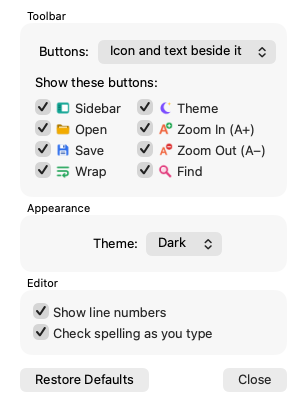
\includegraphics[width=6.5cm]{figures/settings.png}
  \caption{The Settings window, with everything as it starts.}
  \label{fig:settings}
\end{figure}

\begin{center}
\begin{tabularx}{\linewidth}{>{\sffamily}l X l}
  \toprule
  \textbf{Setting} & \textbf{What it does} & \textbf{At first} \\
  \midrule
  Buttons & How toolbar buttons look: \ui{Icon and text beside it},
            \ui{Text under icon} or \ui{Icon only}. & Icon and text \\
  Show these buttons & Which buttons are on the toolbar. The font and
            language boxes are always shown. & All \\
  Theme & \ui{Dark} or \ui{Light}. & Dark \\
  Show line numbers & The line numbers beside the text. & On \\
  Check spelling as you type & Underlines misspelled words
            (section~\ref{sec:spelling}). Greyed out where it isn't
            available. & On \\
  \bottomrule
\end{tabularx}
\end{center}

\subsection{What \appname\ remembers}\label{sec:remembers}

When you close the window, \appname\ remembers its size and position, the font
and text size, the theme, the word-wrap setting, whether the sidebar is shown
and everything in Settings, and restores them the next time it starts.

It doesn't reopen your files: each time \appname\ starts, it opens a blank
document. If you close the window with unsaved changes, it asks whether to
save them first. Use \menu{File > Open Recent} to get back to recent files
and folders. Passwords are never remembered. Section~\ref{sec:reset} explains how to reset them.

% ---------------------------------------------------------------- Saving
\section{Saving files}\label{sec:saving}

\subsection{Save and Save As}

\begin{itemize}
  \item \menu{File > Save} (\key{⌘S} / \key{Ctrl+S}, or \ui{Save} in the
        toolbar) saves the file under its current name. A new, untitled file
        asks for a name first.
  \item \menu{File > Save As…} (\key{⇧⌘S} / \key{Ctrl+⇧S}) saves under a new
        name. For a new file, the dialog suggests \texttt{untitled.txt} in your
        Documents folder.
\end{itemize}

\subsection{How files are saved}

\appname\ is careful to change only what you edited:

\begin{itemize}
  \item \textbf{Line endings are kept.} A file with Windows-style (CRLF) line
        endings is saved with CRLF; anything else with LF. New files use LF.
  \item \textbf{The encoding is kept.} UTF-8 files are saved as UTF-8 and
        Latin-1 files as Latin-1. Latin-1 can only store 256 different
        characters, so if you have added a character it can't hold, such as
        ``€'' or an emoji, \appname\ asks whether to save the file as UTF-8
        instead. Choose \ui{Cancel} to go back and edit the text.
  \item \textbf{Saves are atomic.} The new text is written to a temporary file
        first and then swapped in. If a save fails, for example because the
        disk is full, the original file is left untouched and a message
        explains what went wrong.
  \item \textbf{Other people's changes are noticed.} If the file was changed
        by another program (or another person, on a server) since you opened
        it, \appname\ says so before saving. Choose \ui{Replace} to save your
        version over theirs, \ui{Reload} to throw away your changes and load
        theirs, or \ui{Cancel}.
\end{itemize}

\subsection{Unsaved changes}\label{sec:unsaved}

If a file has unsaved changes when you close its tab, close the window or
quit, \appname\ asks whether to save them, one tab at a time:

\begin{description}[leftmargin=1.5em]
  \item[\ui{Save}] saves the file, then carries on.
  \item[\ui{Don't Save} / \ui{Discard}] throws the changes away, then carries on.
  \item[\ui{Cancel}] does nothing, so you can keep editing.
\end{description}

\appname\ does not save automatically, so remember to save your work.

% ---------------------------------------------------------------- Folders
\section{Folders and the sidebar}\label{sec:folders}

Open a whole folder to see its files in the sidebar on the left of the window.

\subsection{Opening a folder}

Choose \menu{File > Open Folder…} (\key{⇧⌘O} / \key{Ctrl+⇧O}), drop a folder on
the window or on the Dock icon, pass a folder name on the command line, or pick
one from \menu{File > Open Recent}. The sidebar shows one folder at a time;
opening another replaces it. \menu{File > Close Folder} closes it.

Show or hide the sidebar with \menu{View > Show Sidebar} (\key{⌘\textbackslash}
/ \key{Ctrl+\textbackslash}) or \ui{Sidebar} in the toolbar. Drag its title
to move it to the other side of the window, or out into a separate panel.

\subsection{Using the sidebar}

\begin{itemize}
  \item The folder's full path, or \texttt{sftp://} address, is shown at the
        top.
  \item Click a file to open it in a tab. Click a folder to open or close it.
  \item Folders are listed before files. Hidden files (names starting with a
        dot) are hidden; to show them, click \ui{⋯} at the top of the sidebar
        and choose \ui{Show Hidden Files}.
  \item A local folder updates by itself when files change. A folder on a
        server doesn't, so use \ui{Refresh} (in the \ui{⋯} menu or the
        right-click menu) to see changes made by others.
\end{itemize}

\subsection{File commands}

Right-click in the sidebar for these commands:

\begin{description}[leftmargin=1.5em]
  \item[\ui{New File…}, \ui{New Folder…}] Create an empty file or folder in
    the folder you clicked (or next to the file you clicked). A new file opens
    in a tab.
  \item[\ui{Rename…}] Renames a file or folder. Open tabs follow the file.
  \item[\ui{Move to Trash…} / \ui{Delete…}] On this computer, the item moves
    to the Trash (Recycle Bin), so you can get it back. On a server, it is
    deleted for good, after you confirm; only empty folders can be deleted
    there.
  \item[\ui{Copy Path}] Copies the item's path or \texttt{sftp://} address.
  \item[\ui{Refresh}] Lists the folder again.
\end{description}

% ---------------------------------------------------------------- SFTP
\section{Files on a server (SFTP)}\label{sec:sftp}

\appname\ can open and save files on any server you can reach with SFTP, the
file-transfer part of SSH, which nearly every Linux, macOS and Unix server
offers. It uses your existing SSH setup: the keys in your \texttt{.ssh}
folder, \texttt{ssh-agent} (on macOS and Linux), and the settings in
\texttt{\textasciitilde/.ssh/config}. Section~\ref{sec:sftp-windows} explains
the differences on Windows.

\subsection{Connecting}

\begin{description}[style=nextline, leftmargin=1.5em]
  \item[\menu{File > Connect to Server…} (\key{⌘K} / \key{Ctrl+K})]
    Asks for the server, then opens your starting folder there in the
    sidebar.
  \item[\menu{File > Open Remote File…}]
    Asks for the server, then lets you pick a file to open.
  \item[\menu{File > Open Remote Folder…}]
    Asks for the server, then lets you pick a folder for the sidebar.
\end{description}

In the \ui{Connect to Server} window, fill in the server's name, the port
(usually 22), your user name on the server and, if you like, a starting folder
(your home folder if left empty). Or paste an address such as
\texttt{sftp://alice@example.com:2222/var/www} into \ui{Address}. Tick
\ui{Remember this server} to add it to the \ui{Saved servers} list; only the
address and folder are saved, never a password.

\subsection{Logging in}

\appname\ tries these ways to log in, in order:

\begin{enumerate}
  \item \texttt{ssh-agent}, if it is running and holds a key (macOS and Linux);
  \item your key files: the ones named in \texttt{\textasciitilde/.ssh/config},
        then \texttt{id\_ed25519}, \texttt{id\_ecdsa} and \texttt{id\_rsa}.
        If a key has a passphrase, you are asked for it;
  \item the server's own questions (such as a password and a one-time code),
        or a password.
\end{enumerate}

Passwords and passphrases are used once and forgotten: they are never saved,
and you are asked again if \appname\ has to reconnect.

\subsection{The server's key}

The first time you connect to a server, \appname\ shows the server's key
\emph{fingerprint} and asks whether to trust it. Compare it with the
fingerprint your server's administrator gives you. If you choose \ui{Trust and
Connect}, the key is added to \texttt{\textasciitilde/.ssh/known\_hosts}, the
same file the \texttt{ssh} command uses, and you aren't asked again.

\begin{caution}[If a server's key has changed]
If a server presents a different key from the one recorded, \appname\ refuses
to connect and explains why. This can mean that someone is intercepting the
connection. If you know the key changed for a good reason (for example, the
server was reinstalled), remove the old key, for example with
\texttt{ssh-keygen -R example.com}, and connect again. There is deliberately
no way to connect anyway.
\end{caution}

\subsection{Working with remote files}

Files on a server open in tabs like any other, with the same safeguards
(section~\ref{sec:opening}). Their tabs show the \texttt{sftp://} address when
you point at them.

\begin{itemize}
  \item \textbf{Saving} replaces the file in one step, keeping its
        permissions, so a dropped connection never leaves a half-written file.
        If someone changed the file on the server since you opened it, you are
        asked first (section~\ref{sec:saving}).
  \item \textbf{Save As} for a remote file picks a new name on the same
        server. \menu{File > Save to Server…} saves any file to a server; its
        \ui{This Computer…} button saves locally instead.
  \item \textbf{Slow connections:} if an operation takes more than a moment,
        a progress window appears; \ui{Cancel} stops it.
  \item \textbf{Dropped connections:} your text stays in its tab. When you
        save, \appname\ reconnects (asking for a password if needed) and tries
        again.
\end{itemize}

\begin{note}
A save writes a temporary file named \texttt{.\textit{name}.tetmp-\dots} next
to the file and then swaps it in, so you need permission to create files in
the file's folder. If the connection drops in the middle of a save, that hidden
temporary file may be left behind; it is safe to delete.
\end{note}

\subsection{On Windows}\label{sec:sftp-windows}

On Windows, \appname\ uses the same files as the OpenSSH client built into
Windows, in the \texttt{.ssh} folder of your user folder
(\path{C:\Users\<you>\.ssh}):

\begin{itemize}
  \item your key files (\texttt{id\_ed25519}, \texttt{id\_ecdsa},
        \texttt{id\_rsa}, or those named in \texttt{.ssh\textbackslash config});
  \item \texttt{.ssh\textbackslash config} for host names, ports, user names
        and key files;
  \item \texttt{.ssh\textbackslash known\_hosts} for the servers you trust.
\end{itemize}

The Windows OpenSSH agent (the \ui{ssh-agent} service) isn't used: \appname\
reads keys from the \texttt{.ssh} folder, and asks for a key's passphrase when
it needs one. If you have no key yet, you can create one in a Command Prompt
with \texttt{ssh-keygen -t ed25519}, or log in with a password.

The portable version never writes passwords or passphrases to its
\texttt{settings} folder, so a copy of the folder on a USB stick carries no
secrets. Your \texttt{.ssh} folder stays on the computer, not on the stick.

% ---------------------------------------------------------------- Printing
\section{Printing}

Choose \menu{File > Print…} or press \key{⌘P} / \key{Ctrl+P}. Your system's
print dialog opens. To print only part of the file, select that text first; the
print dialog then offers to print just the selection.

The printout always uses the Light theme's colours, with syntax highlighting,
in the editor's current font, so a dark theme never puts white text on a black
background on paper.

% ---------------------------------------------------------------- Closing
\section{Closing and quitting}

\subsection{Close Tab, Close Window and Quit}

\begin{description}[leftmargin=1.5em]
  \item[\menu{File > Close Tab} (\key{⌘W} / \key{Ctrl+W})] Closes the current
    tab.
  \item[\menu{File > Close Window} (\key{⇧⌘W} / \key{Ctrl+⇧W})] Closes the
    window and all its tabs.
  \item[\menu{Quit} (\key{⌘Q}, or \key{Ctrl+Q} on Linux)] Quits \appname. On macOS,
    Quit is in the \menu{\appname} menu; on Windows and Linux, it's in the
    \menu{File} menu.
\end{description}

Each of these first asks about unsaved changes (section~\ref{sec:unsaved}).

\subsection{On macOS}

Like most Mac apps, \appname\ keeps running in the Dock after you close its
window. It remembers the tabs and folder you had open (section~\ref{sec:remembers})
for the next time it starts, and the window comes back empty. To bring it back,
do any of these:

\begin{itemize}
  \item click the \appname\ icon in the Dock;
  \item drop a file or folder on the Dock icon, which opens it;
  \item choose \menu{File > New Tab} or \menu{File > Open…} from the menu bar.
\end{itemize}

To stop \appname\ completely, choose \menu{\appname{} > Quit \appname}, press
\key{⌘Q}, or Control-click the Dock icon and choose \menu{Quit}.

\subsection{On Windows and Linux}

\appname\ has one window, so closing it also quits the program.

% ---------------------------------------------------------------- Shortcuts
\section{Keyboard shortcut reference}

\begin{center}
\begin{tabularx}{\linewidth}{>{\sffamily}X l l}
  \toprule
  \textbf{Command} & \textbf{macOS} & \textbf{Windows / Linux} \\
  \midrule
  \multicolumn{3}{l}{\textit{File}} \\
  New Tab               & \key{⌘N} or \key{⌘T} & \key{Ctrl+N} or \key{Ctrl+T} \\
  Open                  & \key{⌘O}  & \key{Ctrl+O} \\
  Open Folder           & \key{⇧⌘O} & \key{Ctrl+⇧O} \\
  Connect to Server     & \key{⌘K}  & \key{Ctrl+K} \\
  Save                  & \key{⌘S}  & \key{Ctrl+S} \\
  Save As               & \key{⇧⌘S} & \key{Ctrl+⇧S} \\
  Print                 & \key{⌘P}  & \key{Ctrl+P} \\
  Close Tab             & \key{⌘W}  & \key{Ctrl+W} \\
  Close Window          & \key{⇧⌘W} & \key{Ctrl+⇧W} \\
  Quit                  & \key{⌘Q}  & \key{Ctrl+Q} (Linux) \\
  \midrule
  \multicolumn{3}{l}{\textit{Edit}} \\
  Undo / Redo           & \key{⌘Z} / \key{⇧⌘Z} & \key{Ctrl+Z} / \key{Ctrl+Y} \\
  Cut / Copy / Paste    & \key{⌘X} / \key{⌘C} / \key{⌘V} & \key{Ctrl+X} / \key{Ctrl+C} / \key{Ctrl+V} \\
  Select All            & \key{⌘A}  & \key{Ctrl+A} \\
  Find                  & \key{⌘F}  & \key{Ctrl+F} \\
  Replace               & \key{⌥⌘F} & \key{Ctrl+H} (\key{Ctrl+R} on KDE) \\
  Find Next             & \key{⌘G}  & \key{F3} \\
  Find Previous         & \key{⇧⌘G} & \key{⇧F3} \\
  Go to Line            & \key{⌘L}  & \key{Ctrl+L} \\
  Settings              & \key{⌘,}  & \key{Ctrl+,} \\
  \midrule
  \multicolumn{3}{l}{\textit{View}} \\
  Word Wrap             & \key{⌥Z}  & \key{Alt+Z} \\
  Zoom In               & \key{⌘=}  & \key{Ctrl+=} \\
  Zoom Out              & \key{⌘−}  & \key{Ctrl+−} \\
  Actual Size           & \key{⌘0}  & \key{Ctrl+0} \\
  Show Sidebar          & \key{⌘\textbackslash} & \key{Ctrl+\textbackslash} \\
  Show Preview          & \key{⇧⌘P} & \key{Ctrl+⇧P} \\
  Show as Grid (CSV/TSV) & \key{⇧⌘G} & \key{Ctrl+⇧G} \\
  Next / Previous Tab   & \key{⌃Tab} / \key{⌃⇧Tab} & \key{Ctrl+Tab} / \key{Ctrl+⇧Tab} \\
  \midrule
  \multicolumn{3}{l}{\textit{Find bar}} \\
  Next match            & \key{Return}  & \key{Enter} \\
  Previous match        & \key{⇧Return} & \key{⇧Enter} \\
  Close the find bar    & \key{Esc}     & \key{Esc} \\
  \bottomrule
\end{tabularx}
\end{center}

% ---------------------------------------------------------------- Troubleshooting
\section{Troubleshooting}

\subsection*{Windows says ``Windows protected your PC''}
The Windows version isn't signed. Click \ui{More info}, then \ui{Run anyway}, as
described in section~\ref{sec:install-windows}.

\subsection*{macOS says it can't verify \appname\ or that it is damaged}
This build is not notarised by Apple. Control-click the app and choose
\menu{Open}, or use \ui{Open Anyway} in \menu{System Settings > Privacy \&
Security}, as described in section~\ref{sec:install-mac}.

\subsection*{A file shows strange characters such as ``é''}
The file is probably in an encoding other than UTF-8 or Latin-1, such as
Windows-1252 or UTF-16. \appname\ supports only UTF-8 and Latin-1.

\subsection*{\appname\ asks whether to open a file ``anyway''}
The file is either larger than 50~MB or looks like a binary file. Choose
\ui{Open} if you're sure, or \ui{Cancel}. See section~\ref{sec:opening}.

\subsection*{The text runs off the right edge}
Word wrap is off. Press \key{⌥Z} / \key{Alt+Z} or click \ui{Wrap}.

\subsection*{The highlighting colours look wrong}
Check the language box in the toolbar: a file with an unusual extension may need
its language chosen by hand.

\subsection*{On a Mac, I closed the window and \appname\ is still in the Dock}
That's normal Mac behaviour. Click the Dock icon to get a new window, or press
\key{⌘Q} to quit.

\subsection*{``The host key for \dots\ has changed''}
See section~\ref{sec:sftp}. Don't remove the old key unless you know why it
changed.

\subsection*{I can't log in to a server}
Check that \texttt{ssh} or \texttt{sftp} works from a terminal with the same
user name. \appname\ uses the same keys, \texttt{ssh-agent} (not on Windows)
and \texttt{\textasciitilde/.ssh/config}. On Windows, if your key is only loaded
in the Windows \ui{ssh-agent} service, make sure the key file is also in your
\texttt{.ssh} folder (section~\ref{sec:sftp-windows}). For security, it refuses servers that only
offer outdated encryption (such as CBC ciphers or SHA-1); such servers need
updating.

\subsection*{Saving to a server fails with ``permission denied''}
\appname\ saves by creating a temporary file in the same folder, so it needs
permission to create files there, not just to change the file.

\subsection*{Resetting all settings}\label{sec:reset}
Quit \appname, then delete its settings:

\begin{itemize}
  \item \textbf{macOS:} run \texttt{defaults delete com.sjwrc.TextEditor+} in
        Terminal.
  \item \textbf{Windows (portable version):} empty the \texttt{settings}
        folder in the \appname\ folder. If you removed it, delete this registry key instead:\\
        \path{HKEY_CURRENT_USER\Software\sjwrc\TextEditor+}
  \item \textbf{Linux:} delete \texttt{\textasciitilde/.config/sjwrc/TextEditor+.conf}.
\end{itemize}

The next time it starts, \appname\ uses its default window size, font, theme
and word-wrap setting. This also
forgets the saved servers and the Open Recent list.

% ---------------------------------------------------------------- About
\section{About \appname}

\appname\ \version\ was developed by Sanjeeva Wijeyesakere. To see the version you
are running, choose \menu{\appname{} > About \appname} on macOS or
\menu{Help > About \appname} on Windows and Linux.

\appname\ is free software, released under the GNU Affero General Public
License, version~3 or later. It is built with the
\href{https://www.qt.io/}{Qt framework}, used under the GNU LGPL~v3, and uses
\href{https://www.libssh.org/}{libssh} (GNU LGPL~2.1) and OpenSSL (Apache~2.0)
for SFTP. Bug reports
and contributions are welcome on GitHub at
\href{https://github.com/swijeyes}{github.com/swijeyes}.

\end{document}
